\documentclass[aspectratio=169,10pt]{beamer}
\usepackage{amsmath,amssymb}
\usepackage{booktabs}
\usepackage{graphicx}
\usepackage{listings}
\usepackage{xcolor}
\usepackage{hyperref}

% Theme
\usetheme{Madrid}
\usecolortheme{default}

% Title info
\title{LLM Quantization and Evaluation}
\subtitle{CS290W LLM15 Lecture}
\author{LU Yuzhou}
\date{}

% Code listing style
\definecolor{codebg}{RGB}{245,245,245}
\lstset{
    backgroundcolor=\color{codebg},
    basicstyle=\ttfamily\scriptsize,
    frame=single,
    breaklines=true,
    keywordstyle=\color{blue},
    commentstyle=\color{gray},
    stringstyle=\color{red},
    showstringspaces=false,
    upquote=true,
    literate={__}{{\texttt{\_}\texttt{\_}}}2
             {->}{{$\to$}}2
             {=>}{{$\Rightarrow$}}2,
}

\begin{document}

% Title slide
\frame{\titlepage}

% Slide 1: Overview
\begin{frame}{Lab Overview}
    \textbf{Today's Topics:}
    \begin{enumerate}
        \item \textbf{Quantization Fundamentals}: Outliers, sensitivity analysis
        \item \textbf{Modern Methods}: GPTQ, AWQ, GGUF/K-quants
        \item \textbf{Compression}: Pruning with Wanda
        \item \textbf{Evaluation}: Perplexity, MMLU, GSM8K, hardware metrics
    \end{enumerate}

    \vspace{0.5cm}
    \begin{block}{Why This Matters}
        Quantization reduces model size by 4-8$\times$ while maintaining performance, enabling LLM deployment on edge devices and consumer hardware.
    \end{block}

    \vspace{0.3cm}
    \begin{itemize}
        \item \textbf{Recommended Hardware}: AMD Ryzen AI Halo Processors or NVIDIA GPU with 8GB+ VRAM
        \item \textbf{Environment}: ROCm + PyTorch via AUP Learning Cloud
    \end{itemize}
\end{frame}

% Slide 2: What is Quantization?
\begin{frame}{What is Quantization?}
    \textbf{Definition:} Converting model weights and activations from high-precision to lower-precision formats.

    \vspace{0.3cm}
    \begin{block}{Precision Formats}
        \begin{itemize}
            \item \textbf{FP32/BF16} $\to$ \textbf{INT8/INT4} (weights)
            \item \textbf{FP16} $\to$ \textbf{INT8} (activations)
        \end{itemize}
    \end{block}

    \vspace{0.3cm}
    \textbf{Benefits:}
    \begin{itemize}
        \item \textbf{Memory}: 4$\times$ smaller model (FP32 $\to$ INT8)
        \item \textbf{Bandwidth}: Reduced data transfer
        \item \textbf{Speed}: Faster inference on edge devices
    \end{itemize}

    \vspace{0.3cm}
    \begin{block}{Example: 1B Parameter Model}
        FP32: 4 GB \quad$\to$\quad INT8: 1 GB \quad$\to$\quad INT4: 0.5 GB
    \end{block}
\end{frame}

% Slide 3: Quantization Fundamentals
\begin{frame}{Quantization Fundamentals}
    \textbf{Uniform Quantization Formula:}

    \vspace{0.3cm}
    \begin{block}{Symmetric Quantization}
        \begin{align*}
            \text{scale} &= \frac{\max(|x|)}{q_{\max}} \\
            x_q &= \text{round}\left(\frac{x}{\text{scale}}\right), \text{clipped to } [q_{\min}, q_{\max}] \\
            x_{\text{dequant}} &= x_q \cdot \text{scale}
        \end{align*}
    \end{block}

    \vspace{0.1cm}
    Where:
    \begin{itemize}
        \item $q_{\min} = -(2^{\text{bits}-1})$ (e.g., -128 for INT8)
        \item $q_{\max} = 2^{\text{bits}-1} - 1$ (e.g., 127 for INT8)
    \end{itemize}

    \vspace{0.1cm}
    \textbf{Quantization Error (MSE):}
    $$\text{MSE} = \frac{1}{N}\sum_{i=1}^{N}(x_i - \hat{x}_i)^2$$
\end{frame}

% Slide 4: The Outlier Problem
\begin{frame}{Why Outliers Matter}
    \textbf{Outliers} are extreme values in weights and activations that emerge when models exceed $\sim$6.7B parameters.

    \vspace{0.3cm}
    \begin{block}{Outlier Definition (LLM.int8())}
        A feature dimension $h_i$ is an outlier if:
        \begin{enumerate}
            \item Absolute value $\ge 6$
            \item Appears in $\ge 25\%$ of transformer layers
            \item Appears in $\ge 6\%$ of sequence dimensions
        \end{enumerate}
    \end{block}

    \vspace{0.3cm}
    \textbf{Impact on Quantization:}
    \begin{itemize}
        \item Increase quantization step size $\Delta$, reducing precision for normal values
        \item Concentrate in specific feature dimensions
        \item Critical for contextual knowledge and reasoning
    \end{itemize}

    \vspace{0.3cm}

\end{frame}

% Slide 5: Outliers and Quantization Error
\begin{frame}{Outliers Increase Quantization Error}
    \textbf{Key Insight:} Outliers expand the quantization range, reducing precision for normal values.

    \vspace{0.3cm}
    \begin{table}
        \centering
        \small
        \begin{tabular}{lcccc}
            \toprule
            \textbf{Tensor} & \textbf{Range} & \textbf{Bits} & \textbf{MSE} & \textbf{SNR} \\
            \midrule
            Normal & $[-3.4, 3.4]$ & 8-bit & 0.000062 & 42.16dB \\
            Normal & $[-3.4, 3.4]$ & 4-bit & 0.018200 & 17.50dB \\
            With Outliers & $[-12.1, 16.1]$ & 8-bit & 0.001024 & 33.15dB \\
            With Outliers & $[-12.1, 16.1]$ & 4-bit & 0.284479 & 8.71dB \\
            \bottomrule
        \end{tabular}
    \end{table}

    \vspace{0.5cm}
    \begin{block}{Key Insight}
        Outliers increase the quantization scale, reducing precision for normal values. 4-bit quantization is especially affected.
    \end{block}
\end{frame}

% Slide 6: Layer-wise Sensitivity Analysis
\begin{frame}{Layer-wise Sensitivity Analysis}
    Different layers exhibit varying sensitivity to quantization:

    \vspace{0.3cm}
    \begin{table}
        \centering
        \small
        \begin{tabular}{lll}
            \toprule
            \textbf{Layer Type} & \textbf{Sensitivity} & \textbf{Recommendation} \\
            \midrule
            Input/Embedding & High & Keep in FP16/BF16 \\
            Attention Output & High & Keep in FP16/BF16 \\
            FFN Gate/Down & Medium-High & Consider mixed precision \\
            Bottleneck Layers & Low & Can quantize to INT4 \\
            Output Layers & Moderate & INT8 recommended \\
            \bottomrule
        \end{tabular}
    \end{table}

    \vspace{0.5cm}
    \begin{block}{Mixed-Precision Strategy}
        \begin{itemize}
            \item Keep sensitive layers in higher precision (FP16/BF16)
            \item Aggressively quantize non-sensitive layers (INT4)
            \item Optimize memory without significant accuracy loss
        \end{itemize}
    \end{block}
\end{frame}

% Slide 7: Modern Quantization Methods
\begin{frame}{Modern LLM Quantization Methods}
    \begin{table}
        \centering
        \small
        \begin{tabular}{llll}
            \toprule
            \textbf{Method} & \textbf{Type} & \textbf{Precision} & \textbf{Key Innovation} \\
            \midrule
            \textbf{GPTQ} & PTQ (Weight-Only) & W3A16, W4A16 & Hessian-based compensation \\
            \textbf{AWQ} & PTQ (Weight-Only) & W4A16 & Activation-aware protection \\
            \textbf{SmoothQuant} & PTQ (W\&A) & W8A8 & Migrate outliers to weights \\
            \textbf{LLM.int8()} & PTQ (W\&A) & W8A8 & Mixed-precision for outliers \\
            \textbf{GGUF} & PTQ & Q2\_K to Q8\_0 & K-quants for fine control \\
            \bottomrule
        \end{tabular}
    \end{table}

    \vspace{0.5cm}
    \begin{block}{PTQ vs QAT}
        \begin{itemize}
            \item \textbf{PTQ (Post-Training Quantization)}: After training, using calibration data (no retraining)
            \item \textbf{QAT (Quantization-Aware Training)}: Simulate quantization during training (higher accuracy but expensive)
        \end{itemize}
    \end{block}
\end{frame}

% Slide 8: GPTQ - Hessian-Based Compensation
\begin{frame}{GPTQ: Hessian-Based Compensation}
    GPTQ uses second-order information to minimize quantization error.

    \vspace{0.3cm}
    \textbf{Key Equation:}
    $$\min_q \sum_j H_{ij}(w_j - q_j)^2$$
    where $H$ is the Hessian matrix of the loss function.

    \vspace{0.1cm}
    \textbf{Algorithm:}
    \begin{enumerate}
        \item Process weights column-by-column (or in blocks)
        \item Quantize weight $w_i$ to nearest value $q_i$
        \item Update remaining weights: $w_j \leftarrow w_j - \frac{H_{ij}}{H_{ii}}(w_i - q_i)$
        \item Use Cholesky decomposition for stable Hessian inverse
    \end{enumerate}

    \vspace{0.1cm}
    \begin{block}{Optimizations}
        \begin{itemize}
            \item \textbf{Fixed Order}: Predetermined quantization order
            \item \textbf{Lazy Batch Updates}: Delay updates to batches (e.g., 128 columns)
            \item \textbf{Group Size}: Quantize in groups (e.g., 128) for better tradeoff
        \end{itemize}
    \end{block}
\end{frame}

% Slide 9: GPTQ Results
\begin{frame}{GPTQ: Error Reduction}
    \textbf{GPTQ reduces quantization error by compensating with Hessian information.}

    \vspace{0.3cm}
    \begin{table}
        \centering
        \small
        \begin{tabular}{lc}
            \toprule
            \textbf{Method} & \textbf{4-bit MSE} \\
            \midrule
            Simple Quantization & 0.026443 \\
            GPTQ & 0.013969 \\
            \midrule
            \textbf{Improvement} & \textbf{47.17\%} \\
            \bottomrule
        \end{tabular}
    \end{table}

    \vspace{0.5cm}
    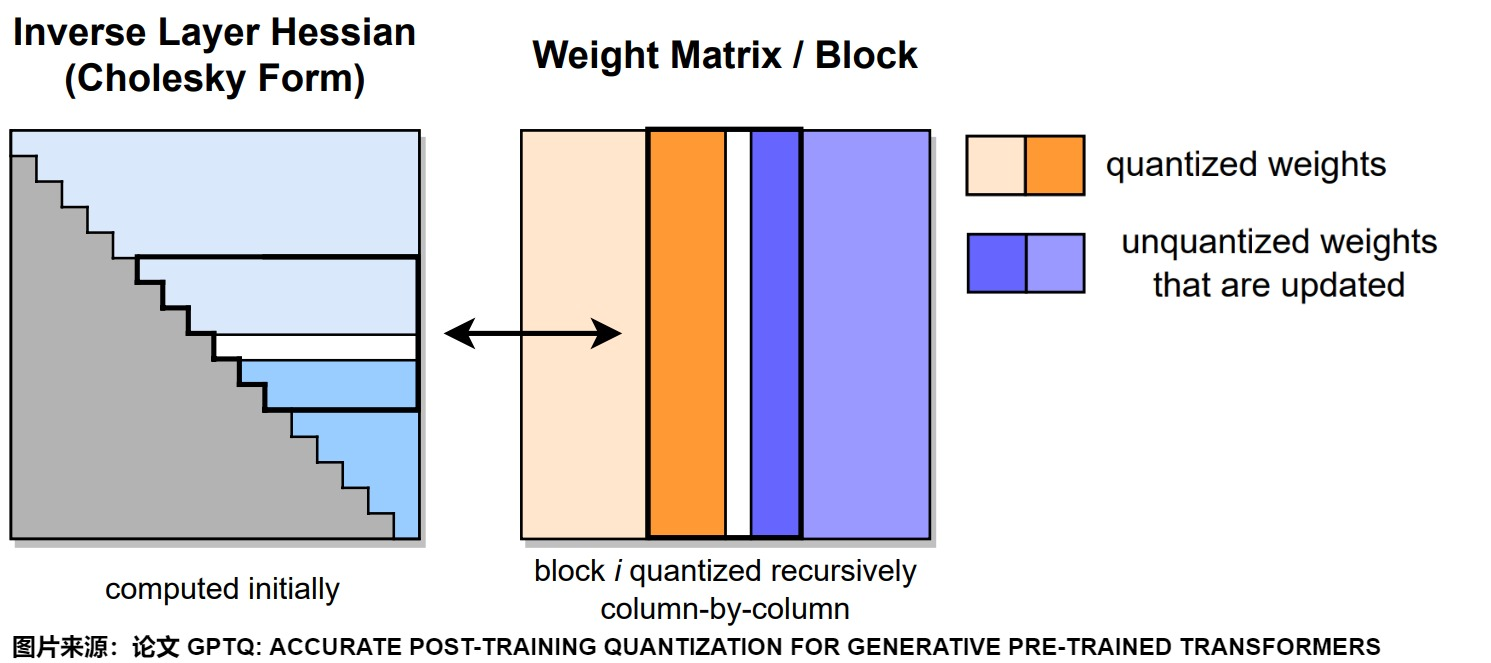
\includegraphics[width=0.8\textwidth]{img/15-gptq.jpg}

    \vspace{0.3cm}
    \begin{block}{Use Case}
        GPTQ is ideal for weight-only quantization (W4A16), best for decoding (IO-bound scenarios).
    \end{block}
\end{frame}

% Slide 10: AWQ - Activation-Aware Weight Quantization
\begin{frame}{AWQ: Activation-Aware Weight Quantization}
    \textbf{Key Insight:} Not all weights are equally important. A small fraction (0.1\%-1\%) of ``salient weights'' dominates model performance.

    \vspace{0.3cm}
    \textbf{Salient Weight Identification:}
    $$\mathcal{S} = \{(i, j) : |\mathcal{X}_j| > \tau\}$$
    where $\mathcal{X}_j$ is the activation of channel $j$.

    \vspace{0.3cm}
    \textbf{Protection Strategy:}
    \begin{align*}
        \mathbf{W}' &= \mathbf{W} \cdot \text{diag}(\mathbf{s}) \\
        \mathbf{X}' &= \mathbf{X} \cdot \text{diag}(\mathbf{s})^{-1}
    \end{align*}

    \vspace{0.3cm}
    \begin{block}{Key Point}
        This keeps the output mathematically equivalent while reducing quantization error for important weights.
    \end{block}
\end{frame}

% Slide 11: AWQ Results
\begin{frame}{AWQ: Error Reduction}
    \textbf{AWQ protects important weights by scaling based on activation magnitude.}

    \vspace{0.3cm}
    \begin{table}
        \centering
        \small
        \begin{tabular}{lc}
            \toprule
            \textbf{Method} & \textbf{4-bit MSE} \\
            \midrule
            Simple Quantization & 0.052326 \\
            AWQ & 0.036199 \\
            \midrule
            \textbf{Improvement} & \textbf{30.82\%} \\
            \bottomrule
        \end{tabular}
    \end{table}

    \vspace{0.5cm}
    \begin{center}
        \fbox{TEXT: Insert diagram showing salient channel identification and scaling}
    \end{center}

    \vspace{0.3cm}
    \begin{block}{Key Insight}
        Channels with high activation are scaled to reduce quantization error. AWQ generally outperforms GPTQ in accuracy retention.
    \end{block}
\end{frame}

% Slide 12: GGUF and K-Quants
\begin{frame}{GGUF and K-Quants}
    GGUF (GPT-Generated Unified Format) is the quantization format used by llama.cpp with \textbf{K-quants} for fine-grained control.

    \vspace{0.3cm}
    \begin{table}
        \centering
        \small
        \begin{tabular}{lll}
            \toprule
            \textbf{Type} & \textbf{Size (7B)} & \textbf{Quality} \\
            \midrule
            Q2\_K & $\sim$2.8 GB & Low \\
            Q3\_K\_M & $\sim$3.8 GB & Medium \\
            Q4\_K\_S & $\sim$4.4 GB & Good \\
            Q4\_K\_M & $\sim$4.7 GB & Very Good \\
            Q5\_K\_M & $\sim$5.5 GB & Excellent \\
            Q6\_K & $\sim$6.0 GB & Near-lossless \\
            Q8\_0 & $\sim$7.0 GB & Virtually lossless \\
            \bottomrule
        \end{tabular}
    \end{table}

    \vspace{0.3cm}
    \begin{block}{K-Quant Nomenclature}
        \begin{itemize}
            \item \textbf{Q4\_K\_S (Small)}: 4-bit uniform
            \item \textbf{Q4\_K\_M (Medium)}: 6-bit for critical tensors (gate\_proj, down\_proj)
        \end{itemize}
    \end{block}
\end{frame}

% Slide 13: Why Mixed Precision in K-Quants?
\begin{frame}{Why Mixed Precision in K-Quants?}
    Similar to sensitivity analysis, K-quants recognize that some tensors are more important:

    \vspace{0.3cm}
    \begin{itemize}
        \item \textbf{Attention output tensors}: Critical for context understanding
        \item \textbf{FFN gate/down projections}: Important for reasoning
        \item \textbf{Embedding layers}: Sensitive to quantization
    \end{itemize}

    \vspace{0.3cm}
    \begin{block}{Example: Q4\_K\_M}
        Uses 6-bit for critical tensors while keeping 4-bit for others, achieving better quality with minimal size increase.
    \end{block}

    \vspace{0.3cm}
    \textbf{Key Features:}
    \begin{itemize}
        \item Per-tensor quantization with different bit-widths
        \item Optimized for CPU inference
        \item Supports partial GPU offloading
        \item Efficient memory mapping for fast loading
    \end{itemize}
\end{frame}

% Slide 14: LLM Compression and Pruning
\begin{frame}{LLM Compression and Pruning}
    \textbf{Pruning} removes redundant parameters to reduce model size and computation.

    \vspace{0.3cm}
    \begin{table}
        \centering
        \small
        \begin{tabular}{lll}
            \toprule
            \textbf{Type} & \textbf{Method} & \textbf{Result} \\
            \midrule
            \textbf{Unstructured} & Remove individual weights & Sparse matrices \\
            \textbf{Structured} & Remove rows/columns/heads & Dense smaller matrices \\
            \bottomrule
        \end{tabular}
    \end{table}

    \vspace{0.5cm}
    \textbf{Wanda: Pruning by Weights and Activations}

    \vspace{0.2cm}
    \textbf{Importance Score:}
    $$\mathcal{I}_{i,j} = |\mathbf{W}_{i,j}| \cdot \|\mathbf{X}_j\|_2$$

    \vspace{0.3cm}
    \begin{block}{Advantages}
        \begin{itemize}
            \item No training required (PTQ-compatible)
            \item Works well with quantization
            \item Preserves model performance better than magnitude-only pruning
        \end{itemize}
    \end{block}
\end{frame}

% Slide 15: Wanda Pruning Demo
\begin{frame}[fragile]{Wanda Pruning Demo}
    \textbf{Algorithm:}
    \begin{enumerate}
        \item Compute importance scores: $|W| \cdot \|X\|_2$
        \item For each output neuron, prune weights with lowest importance
        \item Maintain sparsity ratio (e.g., 50\% pruning)
    \end{enumerate}

    \vspace{0.3cm}
    \begin{block}{Example Results}
        \begin{itemize}
            \item Sparsity 30\%: Output MSE = 3.80
            \item Sparsity 50\%: Output MSE = 18.67
            \item Sparsity 70\%: Output MSE = 57.81
        \end{itemize}
    \end{block}

    \vspace{0.3cm}
    \textbf{Combined Approach:}
    \begin{enumerate}
        \item Apply Wanda pruning (e.g., 50\% sparsity)
        \item Quantize remaining weights to INT4 using AWQ/GPTQ
        \item Result: $\sim$8$\times$ compression (2$\times$ from pruning, 4$\times$ from quantization)
    \end{enumerate}
\end{frame}

% Slide 16: Evaluation Methodologies
\begin{frame}{Evaluation Methodologies}
    \textbf{Three Categories of Metrics:}

    \vspace{0.3cm}
    \begin{enumerate}
        \item \textbf{Intrinsic Metrics}: Perplexity (PPL)
        \item \textbf{Extrinsic Benchmarks}: MMLU, GSM8K, ARC, HellaSwag
        \item \textbf{Hardware Metrics}: TPS, Latency, VRAM
    \end{enumerate}

    \vspace{0.5cm}
    \begin{block}{Perplexity Formula}
        $$\text{PPL} = \exp\left(-\frac{1}{N}\sum_{i=1}^{N}\log P(w_i|w_{1:i-1})\right)$$
        \begin{itemize}
            \item Lower perplexity = better language modeling
            \item Typical: 10-20 (excellent), 20-50 (good), 50+ (needs improvement)
            \item Quantized models should have <5\% PPL increase vs. baseline
        \end{itemize}
    \end{block}
\end{frame}

% Slide 17: Perplexity Interpretation
\begin{frame}{Perplexity Interpretation}
    \begin{table}
        \centering
        \small
        \begin{tabular}{ll}
            \toprule
            \textbf{PPL Range} & \textbf{Quality} \\
            \midrule
            < 10 & Exceptional (human-level) \\
            10-20 & Excellent \\
            20-50 & Good \\
            50-100 & Fair \\
            > 100 & Poor \\
            \bottomrule
        \end{tabular}
    \end{table}

    \vspace{0.5cm}
    \begin{block}{Quantization Impact on PPL}
        \begin{itemize}
            \item 4-bit quantization: +2-5\% PPL increase
            \item 8-bit quantization: <1\% PPL increase
            \item AWQ/GPTQ preserve PPL better than naive quantization
        \end{itemize}
    \end{block}
\end{frame}

% Slide 18: MMLU Benchmark
\begin{frame}{MMLU Benchmark}
    \textbf{MMLU (Massive Multitask Language Understanding):}
    \begin{itemize}
        \item 57 tasks across STEM, humanities, and professional domains
        \item 15,908 multiple-choice questions
        \item Measures knowledge and reasoning
        \item Score: Accuracy percentage (0-100\%)
    \end{itemize}

    \vspace{0.5cm}
    \begin{block}{Expected Scores for Qwen3-0.6B}
        \begin{itemize}
            \item BF16 (baseline): $\sim$35-45\%
            \item 4-bit AWQ: $\sim$33-43\% (2-3\% drop)
            \item 4-bit GPTQ: $\sim$32-42\% (3-4\% drop)
            \item 8-bit: $\sim$34-44\% (<1\% drop)
        \end{itemize}
    \end{block}

    \vspace{0.3cm}
    {\footnotesize For comparison, larger models (4B+) score 65-80\%}
\end{frame}

% Slide 19: GSM8K and Other Benchmarks
\begin{frame}{GSM8K and Other Benchmarks}
    \textbf{GSM8K (Grade School Math 8K):}
    \begin{itemize}
        \item 8,500 grade school math problems
        \item 2-8 reasoning steps per problem
        \item Measures mathematical reasoning
        \item Score: Accuracy percentage (0-100\%)
    \end{itemize}

    \vspace{0.3cm}
    \textbf{Other Important Benchmarks:}
    \begin{itemize}
        \item \textbf{ARC}: Science questions (Easy + Challenge)
        \item \textbf{HellaSwag}: Commonsense reasoning
        \item \textbf{TruthfulQA}: Hallucination resistance
        \item \textbf{Winogrande}: Pronoun resolution
    \end{itemize}

    \vspace{0.3cm}
    \begin{center}
        \fbox{TEXT: Insert chart comparing benchmark scores across quantization methods}
    \end{center}
\end{frame}

% Slide 20: Hardware Performance Metrics
\begin{frame}{Hardware Performance Metrics}
    \textbf{Key Metrics:}

    \vspace{0.3cm}
    \begin{enumerate}
        \item \textbf{Token Throughput (TPS)}: Tokens generated per second
        \begin{itemize}
            \item Higher is better; Typical: 20-100 tokens/s
        \end{itemize}

        \item \textbf{Latency}: Time to first token + time per token
        \begin{itemize}
            \item Prefill latency: Process input prompt
            \item Decode latency: Per generated token
        \end{itemize}

        \item \textbf{VRAM Occupancy}: GPU memory usage
    \end{enumerate}

    \vspace{0.5cm}
    \textbf{VRAM Calculation:}
    \begin{align*}
        \text{VRAM} &= \text{Model Size} + \text{KV Cache} + \text{Overhead} \\
        \text{Model Size} &= \text{Parameters} \times \text{Bytes per parameter}
    \end{align*}
\end{frame}

% Slide 21: Performance Comparison
\begin{frame}{Performance Comparison}
    \begin{table}
        \centering
        \small
        \begin{tabular}{lcccc}
            \toprule
            \textbf{Metric} & \textbf{BF16} & \textbf{4-bit AWQ} & \textbf{4-bit GPTQ} & \textbf{GGUF Q4\_K\_M} \\
            \midrule
            VRAM & $\sim$8 GB & $\sim$3 GB & $\sim$3 GB & $\sim$3 GB \\
            TPS & 50-80 & 80-120 & 70-100 & 30-50 (CPU) \\
            PPL & baseline & +2-3\% & +3-5\% & +3-4\% \\
            MMLU & baseline & -2-3\% & -3-4\% & -3-4\% \\
            \bottomrule
        \end{tabular}
    \end{table}

    \vspace{0.5cm}
    \begin{block}{Key Takeaways}
        \begin{itemize}
            \item 4-bit quantization reduces model size by 60-70\% with minimal quality loss
            \item AWQ generally provides better accuracy than GPTQ at 4-bit
            \item GGUF Q4\_K\_M offers excellent CPU inference performance
            \item Mixed-precision (K-quants) preserves quality for sensitive tensors
        \end{itemize}
    \end{block}
\end{frame}

% Slide 22: Summary
\begin{frame}{Summary: Key Takeaways}
    \begin{enumerate}
        \item \textbf{Quantization Fundamentals}: Outliers significantly impact low-bit quantization; sensitivity analysis guides mixed-precision strategies

        \item \textbf{Modern Methods}:
        \begin{itemize}
            \item GPTQ: Hessian-based error compensation (47\% error reduction)
            \item AWQ: Activation-aware weight protection (31\% error reduction)
            \item GGUF: K-quants for fine-grained CPU inference
        \end{itemize}

        \item \textbf{Pruning}: Wanda combines weights and activations for effective sparsity

        \item \textbf{Evaluation}: Use perplexity, MMLU, GSM8K, and hardware metrics together

        \item \textbf{Best Practices}:
        \begin{itemize}
            \item 4-bit AWQ for GPU inference (best accuracy/size tradeoff)
            \item GGUF Q4\_K\_M for CPU inference
            \item Always evaluate on your target tasks
        \end{itemize}
    \end{enumerate}
\end{frame}

% Slide 23: Experiment Further
\begin{frame}{Experiment Further}
    \begin{itemize}
        \item Quantize Qwen3-0.6B using AutoGPTQ, AutoAWQ, and llama.cpp
        \item Compare 4-bit vs 8-bit quantization on your downstream tasks
        \item Apply Wanda pruning before quantization for additional compression
        \item Benchmark TPS and VRAM on your hardware
        \item Evaluate on MMLU subsets relevant to your use case
    \end{itemize}

    \vspace{0.5cm}
    \begin{block}{Resources}
        \begin{itemize}
            \item \textbf{GPTQ Paper}: \href{https://arxiv.org/abs/2210.17323}{arXiv:2210.17323}
            \item \textbf{AWQ Paper}: \href{https://arxiv.org/abs/2306.00978}{arXiv:2306.00978}
            \item \textbf{Wanda Paper}: \href{https://arxiv.org/abs/2306.11695}{arXiv:2306.11695}
            \item \textbf{llama.cpp}: \href{https://github.com/ggerganov/llama.cpp}{GitHub}
            \item \textbf{Lab Notebook}: \texttt{LLM15-Quantization-and-Evaluation.ipynb}
        \end{itemize}
    \end{block}
\end{frame}

\end{document}
